\section{Multi-Core Architecture}
\label{sec:architecture_multicore}
Embedded systems continue to explode in
complexity and functionality~\cite{sld_complexity}. To meet
the size, weight, and power (SWaP) concerns, the advent of
affordable embedded multi-core
processors~\cite{multithreading_multicore,multithreading_multicore_parallelism} 
offer designers the opportunity to achieve better performance 
than single-core processors.
Figure~\ref{fig:introduction:multi_core} illustrates the
architecture of a general-purpose multi-core. In pursuit of
increasing average-case performance, the cores typically
include speculative 
features~\cite{multithreading_cpu_overview} such as
out-of-order execution, branch prediction, data forwarding,
superscalar execution, and 
on-chip caches. However, such optimizations can cause
\emph{timing anomalies}~\cite{LundqvistS99} where a local
worst-case execution time does not lead to the program's
worst-case execution time. Thus, speculation leads to the
degradation of time-predictability and is undesirable for embedded systems.
The PREcision Timed (PRET) machine~\cite{pret_pret,pret_repeatable_timing} and
PRedictability Of Multi-Processor Timing
(PROMPT)~\cite{multithreading_designing_predictable_considerations,KastnerSPCGHF12} 
design philosophies aim to tackle this issue by advocating the
design of \emph{predictable hardware architectures}, while
not sacrificing performance. In particular, the architecture
should provide \emph{timing isolation} between the cores,
i.e., the actions of the cores must not influence each
other's timing behavior. The architecture should be
\emph{timing compositional}, i.e., with repeatable timing behavior
and free of timing anomalies. The following are examples
of unpredictable hardware features with possible predictable
alternatives~\cite{wcet_future_architectures,multithreading_designing_automotive,multithreading_predictable_multiprocessor}:
\begin{itemize}
	\item \emph{Replace caches with fast software managed memories, called scratchpads~\cite{memory_scratchpad_predictable}.}
		  The selection of data and instructions to be allocated to a scratchpad is determined entirely at 
		  compile time~\cite{memory_scratchpad_known_size,memory_scratchpad_concurrent_allocation,KimBCS14,PrakashP13a,memory_scratchpad_unknown_size}. 
		  In the static allocation scheme, the contents of the scratchpad cannot be changed at runtime. In the
		  dynamic allocation scheme, the contents of the scratchpad can be changed at runtime by using compile time decisions.
		  Importantly, the replacement policy of scratchpads is controllable, whereas with caches the replacement policy is controlled by 
		  the hardware, sometimes with unpredictable behaviors (e.g., with the PLRU policy).
		  The memory address spaces of scratchpads and global memory are mutually exclusive. 
		
	\item \emph{Replace out-of-order execution with better code generation from the compiler~\cite{wcet_aware_framework,SchranzhoferPCTC11,memory_multicore_code_positioning,memory_shared_cache_aware_wcrt,pret_merasa}.}
		  A processor's ability to reorder a group of instructions is limited by the size of
		  its instruction buffer. The compiler does not have this limitation because
		  it has access to the entire program and can make better judgments when reordering
		  instructions. However, it may not have the runtime execution information which may affect the performance.

	\item \emph{Deactivate high-performance bus features, such as burst transfers or pipelining, 
		  and use fair time-sharing arbitration policies, such as round-robin or time
		  division multiple access (TDMA)~\cite{memory_tdma_priority_division}.}
		  The round-robin policy cycles through a static list of 
		  cores, granting them access to the bus. If the granted core does not need the bus, then
		  the grant is given to the next core on the list. The TDMA policy cycles through
		  a static list of cores, granting them access for a fixed amount of time 
		  (a time slot), whether the core needs it or not. 
		  If the granted core does not need the bus, then some 
		  policies~\cite{memory_tdma_priority_division,memory_buses,memory_tdma_lottery,memory_arbitration_performance,HamannE05} will 
		  grant the slot to the other cores in a round-robin manner, thus 
		  improving the throughput. Fairness of the arbitration is important to ensure 
		  that all accesses complete within a bounded length of time.
\end{itemize}
Embedded systems designed using the PRET~\cite{pret_repeatable_timing} or PROMPT~\cite{KastnerSPCGHF12}
philosophies are simpler to understand, model, and analyze.
Many predictable single-core processors have been proposed,
such as the %Multiple Active Context System 
MACS~\cite{pret_macs}, 
%Microprogrammed Coarse Grained Reconfigurable Processor 
MCGREP~\cite{pret_mcgrep}, Patmos~\cite{pret_patmos}, %PRET ARM
PTARM~\cite{LiuRBZL12}, and FlexPRET~\cite{ZimmerBSL14} processors.
%Multi-Core Execution of Hard Real-Time Applications Supporting Analysability 
MERASA~\cite{pret_merasa} is a 
predictable multi-core processor that supports hard and non-real-time
threads. Hard real-time threads access scratchpads for predictability, 
while non-real-time threads access caches for performance. An analyzable
memory controller is used to arbitrate shared bus accesses from the cores.
For Java programs, there is the %Java Optimized Processor 
JOP~\cite{pret_java_architecture} processor and its multi-core 
variant~\cite{pret_jop_cmp_scalability} that uses scratchpads and 
a shared TDMA bus.

\begin{figure}
	\centering
	
	\begin{minipage}[t]{0.45\columnwidth}
		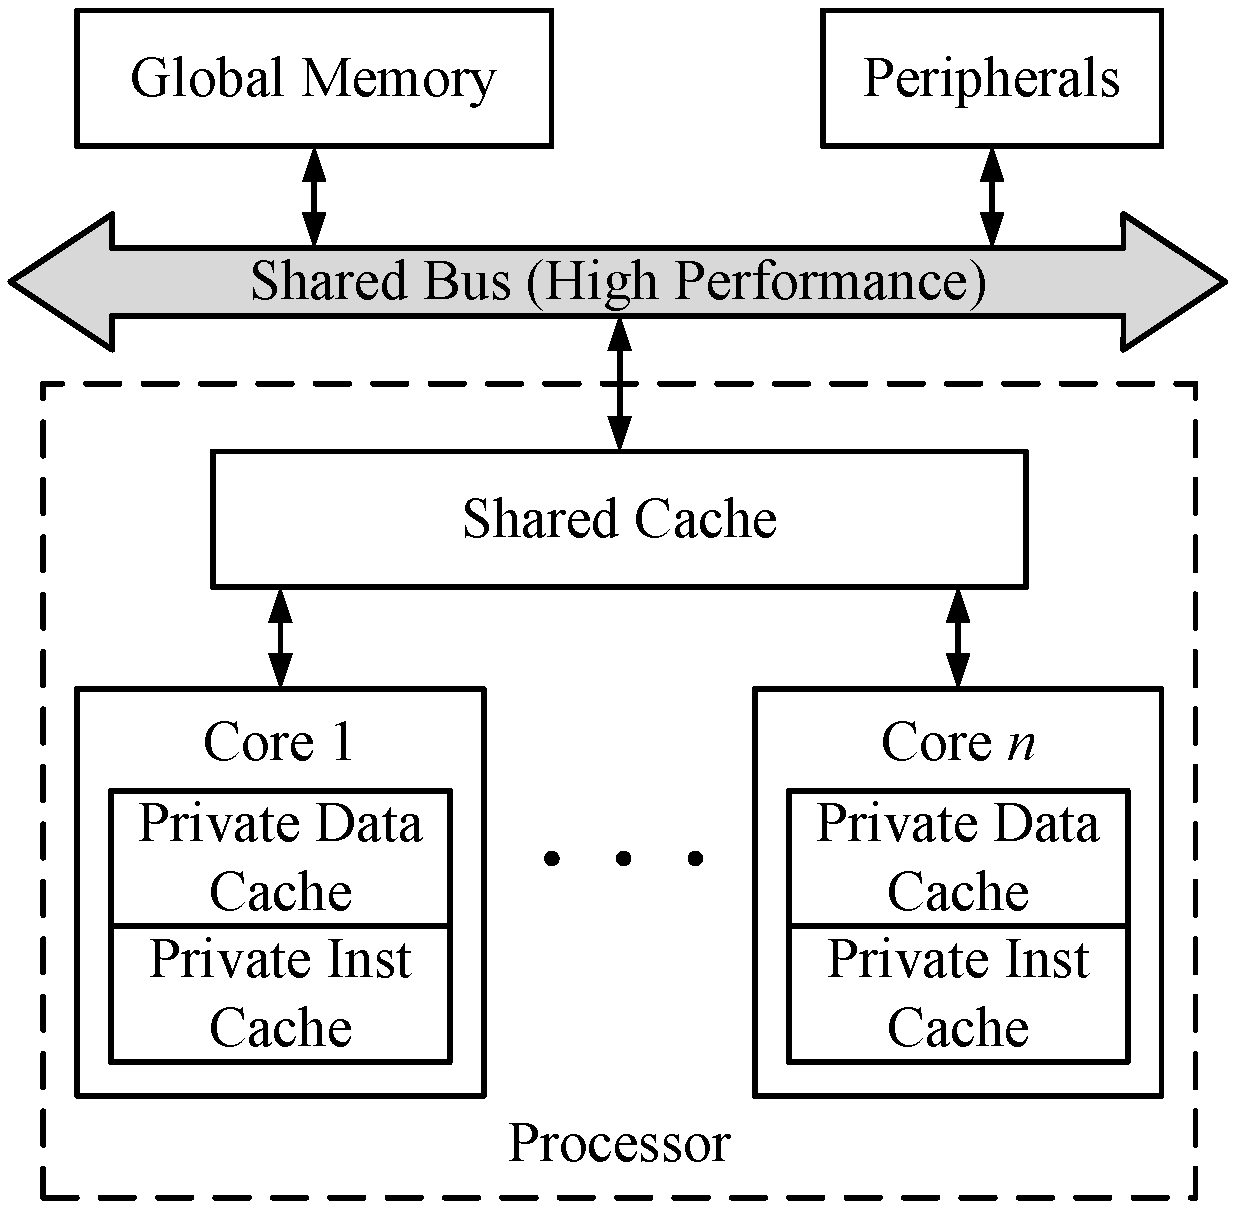
\includegraphics[width=\textwidth]{multi_core}
		\caption{General multi-core architecture.}
		\label{fig:introduction:multi_core}
	\end{minipage}
	\hfill
	\begin{minipage}[t]{0.45\columnwidth}
		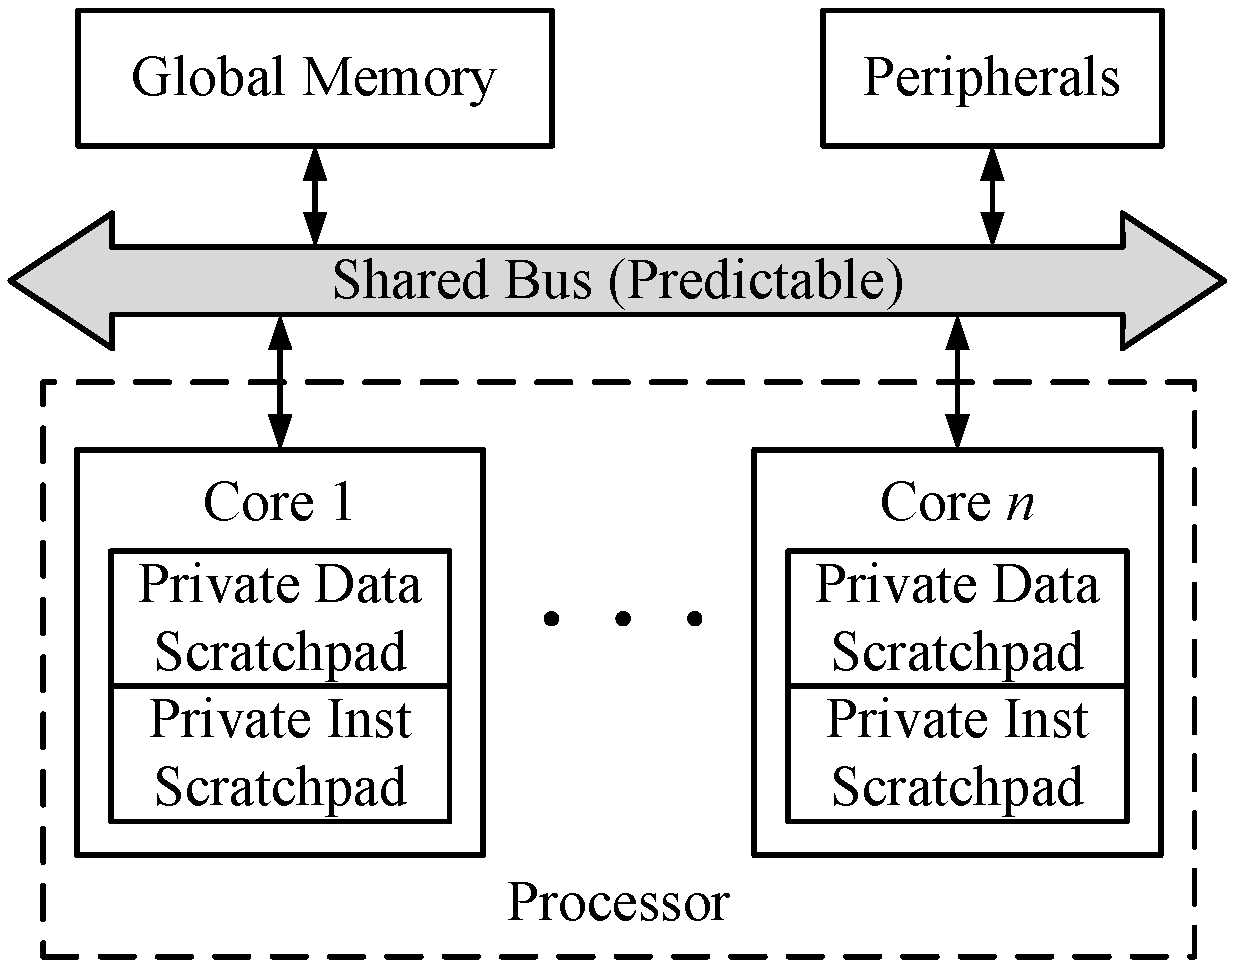
\includegraphics[width=\columnwidth]{multi_core_embedded}
		\caption{Example of a predictable multi-core embedded architecture.}
		\label{fig:introduction:multi_core_embedded}
	\end{minipage}
\end{figure}

The execution of synchronous programs can be accelerated by
\emph{reactive processors}~\cite{SalcicBB02,LiH12}, which
have hardware support for signal resolution, concurrency,
preemptions, and global tick synchronization. A key feature
is their ability to execute programs in a time predictable
manner. Single-core multi-threaded reactive processors
include %Kiel Esterel Processor 
KEP~\cite{LiH12} and %Simultaneous multiThreaded
%Auckland Reactive Processor 
STARPro~\cite{YuanAYRS09}.
Reactive multi-processors include %Embedded
%MultiProcessor supporting Esterel Reactive OpeRations
EMPEROR~\cite{DayaratneRS06} and %HybriD Reactive Architecture 
HiDRA~\cite{SalcicHRB06}. However, these
reactive processors and associated compilers do not support
the execution of host functions written in a host language,
such as C. As a compromise between efficiency and host 
language support, a general purpose processor can be
patched with a reactive functional unit to accelerate the
execution of synchronous constructs. The %Auckland Reactive PRET 
ARPRET~\cite{AndalamRG10} processor is a
patched Xilinx MicroBlaze~\cite{microblaze} processor tailored for executing \pretc{}. 
Java-based reactive single-core processors include %Reactive JOP 
RJOP~\cite{NadeemBS11} and %Tandem Processor JOP 
TP-JOP~\cite{LiMS14}.  %GALS Heterogeneous Multiprocessor 
GALS-HMP~\cite{SalcicM13} is a Java-based reactive multi-processor.

\subsection{Predictable Embedded Multi-Core Architecture}
\label{sec:introduction:pret:multicore}
The architecture of the predictable multi-core used in this 
paper is representative of existing designs.
It is a homogeneous multi-core 
processor~\cite{multithreading_designing_predictable_considerations,pret_java_architecture}
that we have designed using identical Xilinx MicroBlaze~\cite{microblaze} cores, 
illustrated in Figure~\ref{fig:introduction:multi_core_embedded}. 
Each MicroBlaze core has a three-stage, in-order, timing anomaly-free pipeline 
connected to private data and instruction scratchpads.
The scratchpads are statically allocated and loaded at compile time. A shared 
bus with TDMA arbitration connects 
the cores to shared resources, such as global memory and peripherals. Due to 
the resource constraints of existing FPGA devices, we developed a multi-core MicroBlaze
simulator for benchmarking 
purposes. We extended an existing MicroBlaze simulator~\cite{mb_simulator} 
significantly to support cycle-accurate simulation, an arbitrary number of cores, 
and a shared bus with TDMA arbitration.
